\chapter{Improvements}

In case of articulated objects with a skeleton structure, the segmentation algorithm in its simple form fails. The main reasons are the following:
%%
\begin{itemize}
	\item By recursively subdividing $C_1$ and $C_2$ the detected sub clusters might actually count to more than one and being located apart from each other. 
	\item In case of a matching cluster being a part of a rigid part, no further operations are done with the match. The rigid part is anticipated to be generated by merging neighboring sub clusters.
	\item By further sub dividing clusters, the merging becomes more difficult, as the clusters are scattered next to each other.
	\item The detection of joints is not exact although the segmentation in the approximate rigid parts succeeds as sub clusters are good enough to fit, but still there might be better fits with less or more points.
\end{itemize}
%%
Thus, the initial approach needs to be extended, which solved the issues being mentioned.

\section{Region growing}
During the segmentation of an object in two different poses, there is the general case that the divided parts being compared do not contain the same number of points. As this state might come to undesirable matching errors, parts with the same sizes could be generated by region growing. This can be e.g. implemented by starting with the most outside point of two poses and grow regions with the same size of points which are then compared. Furthermore, the detection of multiple clusters can be treated, in case of subdividing clusters. The detected clusters are as a result treated individually.

\section{Matching error}
Another improvement is the assurance that during the ICP procedure each point only has one nearest neighbor and also considering the case, that there are not always the same amount of points in two clusters (uneven number of points). By doing so, not all points would contribute to the matching error. Furthermore, weights should be added to the points, especially points located near a joint should be treated cautiously. A cluster could be therefore further subdivided, if a minimum number of points is above the error threshold $\tau$ and not the average. 

%\section{Initial alignment of clusters}
%The initial ``Divide and Conquer'' approach is used to detect two matching sub clusters of $C_1$ and $C_2$. But unlike previous implementations, the rigid parts are not detected by a following merging step, but by region growing, until the matching error $e$ is above the specified threshold $\tau$.
%If a rigid part is detected, it is stored and the same procedures initiates with the other points of $C_1$ and $C_2$. By doing so, all rigid parts are sequentially detected from one direction to the other.

%\subsection{Error handling}
%The region growing procedure needs to terminate if points of another rigid part are added. Following, a higher matching error $e$ is detected. To guarantee successful rigid part detection this procedure premises that the regions in two comparing sub clusters grow the same way, otherwise the region growing might terminate before detecting the whole rigid part. 

\section{Segmentation of articulated objects}
The most crucial deficit  of the proposed algorithm is that is does not work with articulated objects, whose parts are not simple linked as a chain, but a rigid part can have more than two linking rigid parts. An example would be the skeleton of humans and most animals. As a result, the objects are simply too complex to linearly subdivide them. One improvement proposition is thereby the initial alignment of the object, that the largest rigid part is aligned.  A similar approach was taken during the LRP algorithm \cite{guo2016correspondence}. Then, recursively linked parts of this largest rigid part are detected (see section \ref{LRP}).

\section{Largest rigid part}
\label{LRP}

As opposed to recursively subdividing $C_1$ and $C_2$ into sub clusters, as an initial step the largest rigid part (LRP) is detected. From there, all other linked parts can be detected by region growing and reapplying the algorithm.
The algorithm was applied on 3D point clouds by \ref{LRP}.

\subsection{Basic functionality}
\label{functionalityLRP}
As an initial step, the LRP algorithm  attempts to detect the most reliable correspondences between $C_1$ and $C_2$. For that, local descriptors (FPFH) are computed. The requirement for a sparse correspondence between two cluster points $\boldsymbol{p}_i(x,y)$ and $\boldsymbol{p}_j(x,y)$ is that they are \textit{reciprocal}, which means that two points $\boldsymbol{p}_i(x,y)$ and $\boldsymbol{p}_j(x,y)$ are the most similar from each other. Some of the sparse correspondences are assumed to be wrong. Therefore, by applying RANSAC to the point correspondences, a single rigid transformation is aimed for to detect the so-called ``largest rigid part'' (LRP), which is supported by the largest corresponding point cluster between $C_1$ and $C_2$. In case of a human, this would be the torso. Subsequently, all linked rigid parts to the LRP are detected by recursively applying the algorithm on grown clusters from the current LRP.

\subsection{Implementation steps}

In order to re-implement the algorithm in 2D, modifications had to be accomplished. The most crucial part of the whole algorithm is the initial alignment of $C_1$ and $C_2$ in order to detect the actual largest rigid part of the articulated object. This step is of particular importance, as the subsequent detection of further rigid parts proceeds from there. Therefore, as first step, sparse correspondences between $C_1$ and $C_2$ have to be detected (see subsection \ref{correspondences}). The initial idea was to detect correspondences by applying the ICP only proceeding the iterative transformation calculation with the most reliable correspondences. However, this approach did not manage to detect the desired correspondences of the largest rigid part (see section \ref{ResultsLRP}). Building on the reference paper by Mitra \cite{Mitra07} features for all points of $C_1$ and $C_2$ are computed to use those for point correspondences between two clusters $C_1$ and $C_2$.

\begin{enumerate}
	\item The PCA is employed on the input clusters $C_1$ and $C_2$ to estimate normals of all points.
	\item Point features are computed to detect sparse point correspondences between $C_1$ and $C_2$. A Point correspondence between $C_1$ and $C_2$ needs to be \textit{reciprocal}.
	\item The RANSAC approach is applied on those correspondences to detect a $T_j$ that rejects wrong point correspondences. Clusters are detected from all corresponding points by applying region growing.
	\item The LRP is assigned to the resulting biggest point cluster.
	\item Proceeding with the LRP, unmatched clusters to $C_1$ and $C_2$ are seeked by region growing from the LRP. The algorithm is then reapplied on those clusters until all rigid parts have been discovered.
\end{enumerate}

\subsection{Detection of sparse correspondences}
\label{correspondences}

\subsubsection{ICP}
Sparse correspondences of two input clusters $C_i$ and $C_j$ were initially achieved by applying the Iterative closest point algorithm. Thereby, the two input clusters are aligned by means of the PCA. Following, corresponding points of $C_i$ and $C_j$ are only considered, if they are \textit{reciprocal} (see subsection \ref{functionalityLRP}). Furthermore, the euclidean distance between two cluster points $d(\boldsymbol{p}_i,\boldsymbol{p}_j)$ must be below a predefined threshold $\tau$. As a consequence, points being located far away from each other do not contribute to the alignment of $C_i$ and $C_j$ and are not stored as correspondence. Those are assumed to be small rigid parts with different transformations.

\subsubsection{Point features}
As the intermediate results of the detection of the largest rigid part when applying only the ICP were insufficient for further computations (see section \ref{ResultsLRP}) another approach had to be applied. As proposed in \cite{Mitra07} a fast point feature histogram \cite{FPFH} was implemented in 2D. It is an improved approach of the `'Persistent Point Feature Histogram for 3D Point Clouds'' \cite{PPFH}. The choice of those features are the following: 
%%
\begin{itemize}
	\item rotation-invariant features
	\item easy comparison of features
	\item low complex implementation
\end{itemize}
%%
By using a histogram the neighborhoods' geometrical properties can be provided in form of the mean surface curvature at a point $\boldsymbol{p}$. As a first step, the normals of all points from the input clusters $C_1$ and $C_2$ need to be estimated. Those is achieved by taking all points within a radius $r$ from a point $\boldsymbol{p}$. The normals need to be re-oriented and are calculated by using the approach from \cite{normals}. The simplified point feature histogram (SPFH) for a point $\boldsymbol{p}$ is then computed by using three geometric features. Between $\boldsymbol{p}$ and each of its $n$ neighbors $\boldsymbol{p_n}$ given a threshold $\tau$, those features are computed -- $\boldsymbol{p_i}$ is thereby the point having the smaller angle between its normal and the line connecting the point set, $\boldsymbol{p_j}$ the remaining point. Using their normals $n_i$ and $n_j$ a Darboux $uvn$ frame $(u = n_i, v = (p_j - p_i) \times u, w = u \times v)$ is computed. The following angles
%%
\begin{equation}
\begin{split}
\alpha = v \cdot n_j
\\
\phi = (u \cdot (p_j - p_i))/\|p_j - p_j\|
\\
\theta = arctan(w \cdot n_j, u \cdot n_j)
\end{split}
\label{eq:AngularVariations}
\end{equation}
%%
are computed. In a second step for each point $\boldsymbol{p_i}$ again all $n$ neighbor points given a threshold $tau$ are computed. The final histogram of $p$ is then weighted to the final histogram (FPFH)
%%
\begin{equation}
FPFH(\boldsymbol{p}) = SPF(\boldsymbol{p}) + \frac{1}{n} \cdot \displaystyle\sum_{i=1}^{n}\frac{1}{w_i} \cdot SPF(p_i)
\end{equation}
%%
where the weight $w_i$ represents the distance $d(\boldsymbol{p},\boldsymbol{p}_i)$. The influence region diagram for a Fast Point feature histogram for a query point $\boldsymbol{p_q}$ can be seen on Figure \ref{fig:FPFHregion}. 
%%
\begin{figure}[H]
	\centering
	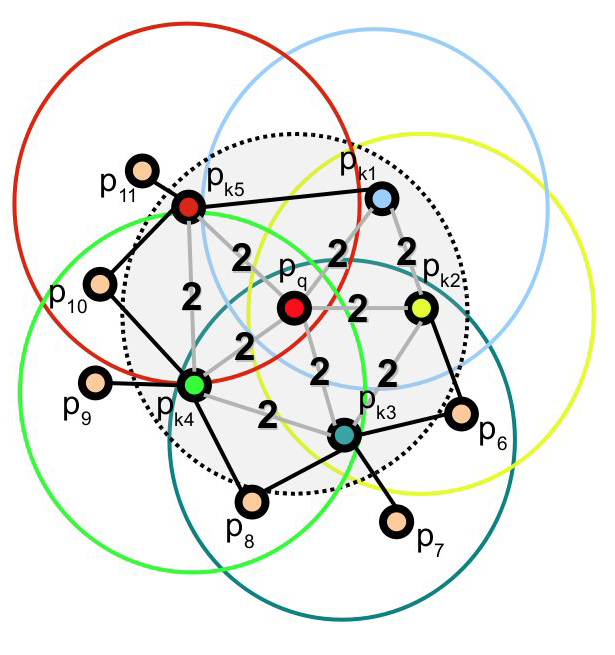
\includegraphics[width=0.4\linewidth]{FPFH_region}
	\caption{The point region for the calculation of the feature histogram for a query point $\boldsymbol{p}_q$. The histogram of $\boldsymbol{p}_q$ and its neighbors (inside the grey circle) is weighted with the further linked neighbors (colored circles).}
	\label{fig:FPFHregion}
\end{figure}
%%
The resulting features are added into histograms with 125 bins. As soon as the feature histograms of all points from $C_1$ and $C_2$ are computed, they can be compared and the most similar histograms are selected as correspondence if they are \textit{reciprocal}. Before, a persistence analysis is computed, which only takes salient histograms for comparison. 

\subsection{Detection of the largest rigid part}
\label{detectionLRP}
The dense point correspondences from the previous computation step (see subsection \ref{correspondences}) may contain several errors. Therefore, RANSAC is applied as a next step to detect a single rigid transformation $T$ that leads to the biggest overlapping point cluster of $C_i$ and $C_j$. Thereby, in each iteration, 3 random correspondences are selected and used for the calculation of $T$ which is applied on $C_i$ to be translated on $C_j$. Subsequently, clusters are grown from all corresponding points with an euclidean distance $d(\boldsymbol{p}_i,\boldsymbol{p}_j)$ again below a predefined threshold $\tau$. The procedure is applied both on $C_i$ and $C_j$ which results in two rigid parts as output. In case of symmetric poses, the RANSAC would not be required, as the largest rigid part (the torso) would be almost perfectly aligned and taken as input for the region growing. But still, to cover as many cases as possible, this computation step is necessary. 

\subsection{Cluster detection by region growing}
\label{cluster}
After successfully detecting a ``largest rigid part'' $P_i$ and $P_j$ for each input clusters $C_i$ and $C_j$ they are added to a list of rigid parts $\mathcal{P}$. Potential linked rigid parts are detected from region growing of all unclustered points $\mathcal{U} =  \{\boldsymbol{u}_1,\ldots,\boldsymbol{u}_n\}$. Those comprise all cluster points of $C_1$ and $C_2$ excluding already detected largest rigid parts $\mathcal{P}$. The region growing initiates with the first point $\boldsymbol{u}_1$ of the unclustered points $\mathcal{U}$ to form a cluster $C_i$. Another point of the unclustered points $\boldsymbol{u}_j$ is added to $C_i$, if the euclidean distance $d(\boldsymbol{p}_i,\boldsymbol{u}_j)$ to any point in $C_i$ is below the threshold $\tau$. If no further unclustered points can be added, the region growing initiates again with the first unclustered point $\boldsymbol{u}_1$ that has not been added by region growing until all points traversed the procedure. The result is a set of clusters $\mathcal{C}$ for each $C_i$ and $C_j$. Subsequently, a preliminary joint $\boldsymbol{j}_i$ for each output clusters is stored, by detecting the two nearest points of $C_i$ and $P_i$. The joints are required for following cluster correspondence and joint weights for the ICP (see subsection \ref{CorrespondingClusters} and \ref{JointWeights}).

\subsection{Establishment of corresponding clusters}
\label{CorrespondingClusters}
In case of detecting more than one cluster for each $C_i$ and $C_j$, which might be for example the case for the extremities linked to the torso, it must be verified which clusters correspond to each other. This step is essential, as the algorithm is called recursively (starting from \ref{correspondences}) with two new input clusters. Thereby, the provisional joints $\boldsymbol{j}_i$ are used to associate two clusters of $C_i$ and $C_j$ by detecting the closest joint with the euclidean distance $d(\boldsymbol{j}_i,\boldsymbol{j}_j)$.

\subsection{Joint weights}
\label{JointWeights}
In order to iteratively detect largest rigid parts that are actually linked to another detected ``largest rigid part'', the preliminary joints resulting from \ref{cluster} are used as weights. Thereby, points being located far away from joints, do not contribute as much to the matching error as point located near a joint. By doing so, joint consistency across two poses is enforced. As an alternative to the ICP clusters with calculated joints only need to be rotated around them. As a result, a matching error $e$ 
%
\begin{equation}
	e = \displaystyle\sum_{i=1}^{m}\| \boldsymbol{p}_i - \boldsymbol{q}_i\|^2 \cdot \| \boldsymbol{p}_i - \boldsymbol{j}_i\|
\end{equation}
%
is achieved which combines the distance to the closest point and to the cluster's joint. Thereby, not only successful correspondences are taken as input but all points, that the error is expressive. The final correspondence equals to the rotation around the joint $\boldsymbol{j}_i$ with the smallest error $e$. 

\section{Implementation}
\label{ImplementationLRP}
The individual steps of the largest rigid part algorithm have also been split in the implementation for better overview. 
%
%TODO: Add code snippets to implementation LRP
%
\subsection{ICP}
One main part of the algorithm is the modified implementation of the ICP using Procrustes fitting to compute a transformation that detects sparse point correspondences. Thereby, only reciprocal correspondences within a specific distance $\tau$ contribute to the calculation. The final point correspondences of $C_i$ and $C_j$ are stored in a \texttt{Map<Integer, Integer>} containing the indices of the corresponding points. This is because the storage of points in the form $\boldsymbol{p}_i(x,y)$ would underly a specific transformation, which is applied during the ICP and initial alignment. For further computations using the RANSAC, no transformations are desired. As the main difficulty is the right initial alignment of the actual largest rigid part (torso) the value of the distance threshold $\tau$ is chosen generously. As a result, a higher number of false point correspondences is detected which has to be compensated by RANSAC (see subsection \ref{RANSAC}).

\begin{lstlisting}
...
for (Map.Entry<Integer, Integer> entry : reference.entrySet()) {
Integer referenceIndex = entry.getKey();
Integer targetIndex = entry.getValue();

	if (target.containsKey(targetIndex) && target.get(targetIndex) == referenceIndex) {
		referencePoints.add(originalReference.get(referenceIndex));
		targetPoints.add(originalTarget.get(targetIndex));
		finalAssociations.put(referenceIndex, targetIndex);
	}
}
...
\end{lstlisting}

\subsection{Image Features}
%
%TODO: implementation of features (incl normals)
%
\subsection{RANSAC}
\label{RANSAC}
The RANSAC algorithm takes the computed dense correspondences between $C_i$ and $C_j$ in form of a \texttt{Map<Integer, Integer>} as input. As a first step, three random correspondences are selected from the map to calculate an affine transformation between the three resulting points from each $C_i$ and $C_j$. The initial orientation and alignment is thereby irrelevant as the transformation $T$ is completely recalculated.

\begin{lstlisting}
public LargestRigidPart(Cluster c_i, Cluster c_j, Map<Integer, Integer> correspondences)
...
points1 = c_i.getPoints();
points2 = c_j.getPoints();
...
private void getRandomPoints(int num) {
	Integer[] keys = correspondances.keySet().toArray(new Integer[0]);
	Integer[] values = correspondances.values().toArray(new Integer[0]);

	for (int i = 0; i < num; i++) {
		index = (int) (Math.random() * correspondances.size());
		randomPoints1.add(points1.get(keys[index]));
		randomPoints2.add(points2.get(values[index]));
	}
}
...
\end{lstlisting}

Similar to the ICP, a closest point procedure with a threshold $\tau$ is conducted. The value is thereby considerably smaller than in the ICP as a right alignment during any iteration is assumed. Unlikely the ICP, no error during the Procrustes fit is accumulated, instead the detected point correspondences are taken as input in the region growing \ref{RegionGrowing} procedure. The biggest cluster is stored and after all iterations returned as largest rigid part.

\subsection{Region growing}
\label{RegionGrowing}
The region growing algorithm is quite similar to the earlier described algorithm (see algorithm \ref{noiseRemoval}). There is also an adaptation, which does not only return the largest cluster, but all clusters above a certain size. The detected clusters are handled in a \texttt{Stack<Cluster>} in case of more than one detected clusters. Thereby, all clusters are pushed on the stack. With each recursion two corresponding cluster $C_i$ and $C_j$ are popped from the stack and taken as input for the whole algorithm. If again more clusters are detected they are pushed on the stack and treated before recently added clusters.

\section{Results}
\label{ResultsLRP}

As the input point cloud of an articulated object is in 2D, the imitation of the object's hull is required. As a consequence, the region growing is much more error-prone, as unlikely in 3D, the points of a rigid part have a considerable lower number of neighbors. In case of a few missing cluster points from a rigid part, it will not be fully detected during the region growing due to the gaps. To counteract this behavior, joints are added to each rigid part, that more links for region growing are available. 

%TODO: add pictures of LRP results

The first main difficulty is the first alignment of the two input clusters $C_1$ and $C_2$. As the execution of the algorithm is only dependent on a succesful alignment, for test cases the assumption was made, that the orientation of the two poses are initially right. The main drawback of the ICP was that the starting position of the two main clusters $C_1$ and $C_2$ had to be ideal that the largest rigid part could be detected. However, this could not be guaranteed as asymmetrical body poses would influence the orientation (see Figure XXX) of the whole cluster $C_1$. As a result, reciprocal point correspondences could not be detected that would lead to the largest rigid part.

\subsection{Main drawbacks}
The main drawback of the algorithm represents the first initial alignment of the two poses of the articulated object. Thereby, it is directly dependent on the symmetry of the pose. The less symmetry the higher the changes that the initial alignment on the largest rigid part might fail. The reason is that the ICP expects a good starting alignment. As it is assumed that the major largest rigid part contributes most to the principal axis and the initial alignment, it would work. But in case of an unbalance of the linked parts, the alignment of the LRP might shift in a certain direction and it might not be detected during the ICP. As a result the whole algorithm fails. Furthermore, touching of rigid parts (e.g. the hand touches the leg) constitute difficulties as the region growing would not detect those as potential linked clusters. 

\subsection{Possible solutions}

A possible solution to the main drawbacks is the usage of point features for the initial alignment. Those are more reliable across two poses than the anticipated symmetry of the points on linked parts. A similar implementation was done in 3D by Mitra \cite{Mitra07} (see section \ref{functionalityLRP}). 

%TODO: Write what fails/main problems/solutions







